\uuid{OscK}
\exo7id{7147}
\titre{exo7 7147}
\auteur{megy}
\organisation{exo7}
\datecreate{2017-05-01}
\isIndication{true}
\isCorrection{true}
\chapitre{Nombres complexes}
\sousChapitre{Géométrie}
\module{Algèbre}
\niveau{L1}
\difficulte{}

\contenu{
\texte{
\'Ecrire en coordonnée complexe  les deux similitudes (directe et indirecte) envoyant les points d'affixes $2$ et $3$ sur ceux d'affixes $i$ et $3i$ et trouver leurs éléments caractéristiques.
}
\indication{Les deux similitudes se déduisent l'une de l'autre par une certaine réflexion.}
\reponse{
Si la similitude est directe, son angle est $\pi/2$, donc la similitude s'écrit $z\mapsto 2i z+ b$ en coordonnée complexe. Comme $s(2)=i$, on en déduit que $4i+b=i$ c'est-à-dire $b=-3i$.

Le point fixe a alors pour affixe $\dfrac{b}{1-2i} = \dfrac{-3i}{1-2i} = \dfrac{6-3i}{5}$.

\begin{center}
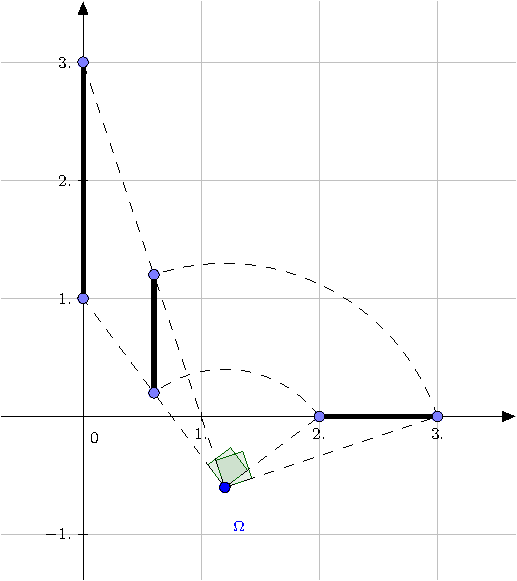
\includegraphics{../images/pdf/OscK-1.pdf}
\end{center}
La similitude indirecte est obtenue en composant la similitude directe précédente par la symétrie d'axe passant par $i$ et $3i$, c'est-à-dire l'axe des ordonnées. Cette symétrie s'écrit $z\mapsto -\bar z$. On en déduit que la similitude indirecte envoyant les points d'affixes $2$ et $3$ sur ceux d'affixes $i$ et $3i$ s'écrit
\[z\mapsto -\overline{(2iz-3i)} = 2i\bar z-3i.
\]
(Alternativement, et sans utiliser la question précédente, on sait d'après l'énoncé que la similitude indirecte doit s'écrire $z\mapsto 2i \overline z + b$, et comme $s(2)=i$, on en déduit bien $i = 4i+b$ d'où $b=-3i$.)

Cette similitude possède un unique point fixe d'affixe $\omega$, solution de l'équation $\omega = 2i\bar\omega -3i$.

On remarque que $\omega$ est donc aussi l'unique point fixe de $s\circ s$, ce qui donne l'équation $\omega = 2i\overline{(2i\bar \omega-3i)} -3i = 4\omega-6-3i$ d'où $\omega = 2+i$.


Finalement, comme on sait que l'axe est dirigé par le vecteur d'affixe $1+i$ et que cet axe passe par le centre de la similitude, cet axe est la droite d'équation $y=x-1$

\begin{center}
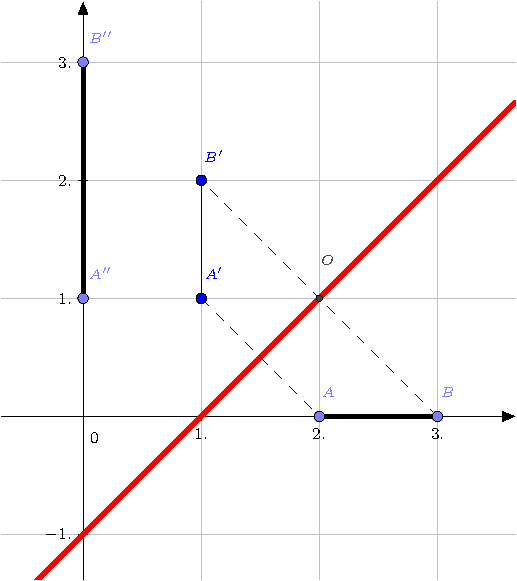
\includegraphics{../images/pdf/OscK-2.pdf}
\end{center}
}
}
